\documentclass[11pt,a4paper]{book}

\usepackage{mypackage} % moje definice a styly


\faculty{Faculty of science}
\department{Department of theoretical physics and astrophysics}
\university{Masaryk University}
\thesisType{Ph.D. Dissertation}
\city{Brno}
\academicYear{2022/2023}
\yearOfMaking{2022}
\thesisTitle{Analysis and Modelling of Non-linear \newline Dynamical Systems in Astrophysics}
\thesisTitleEN{Analysis and Modeling of Non-linear \newline Dynamical Systems in Astrophysics}
\thesisTitleCZ{Analýza a modelování nelineárních dynamických systémů v astrofyzice}
\author{Jiří Květoň}
\authorFull{Mgr. Jiří Květoň}
\supervisor{Mgr. Filip Hroch Ph.D.}
\consultant{Mgr. Viktor Votruba Ph.D.}
\coverImage{./img/cover.png}

% References package defs
\usepackage[
    backend=biber, style=authoryear, citestyle=authoryear, sorting=ynt
]{biblatex}

% References file
% pozn. https://tex.stackexchange.com/questions/305381/biblatex-empty-bibliography ... kvuli chybe nedefinovanych bib
\addbibresource{./references.bib}

\begin{document}
    % Pro uvodni strany se vypne cislovani
    \pagenumbering{gobble}

    % --
    % Titulní strana prace
    % --
    \maketitle
    \blankpage

    % --
    % Originální zadání
    % --
    % scale a offset aby marginy vicemene sedely do rozmeru ostatnich stranek
    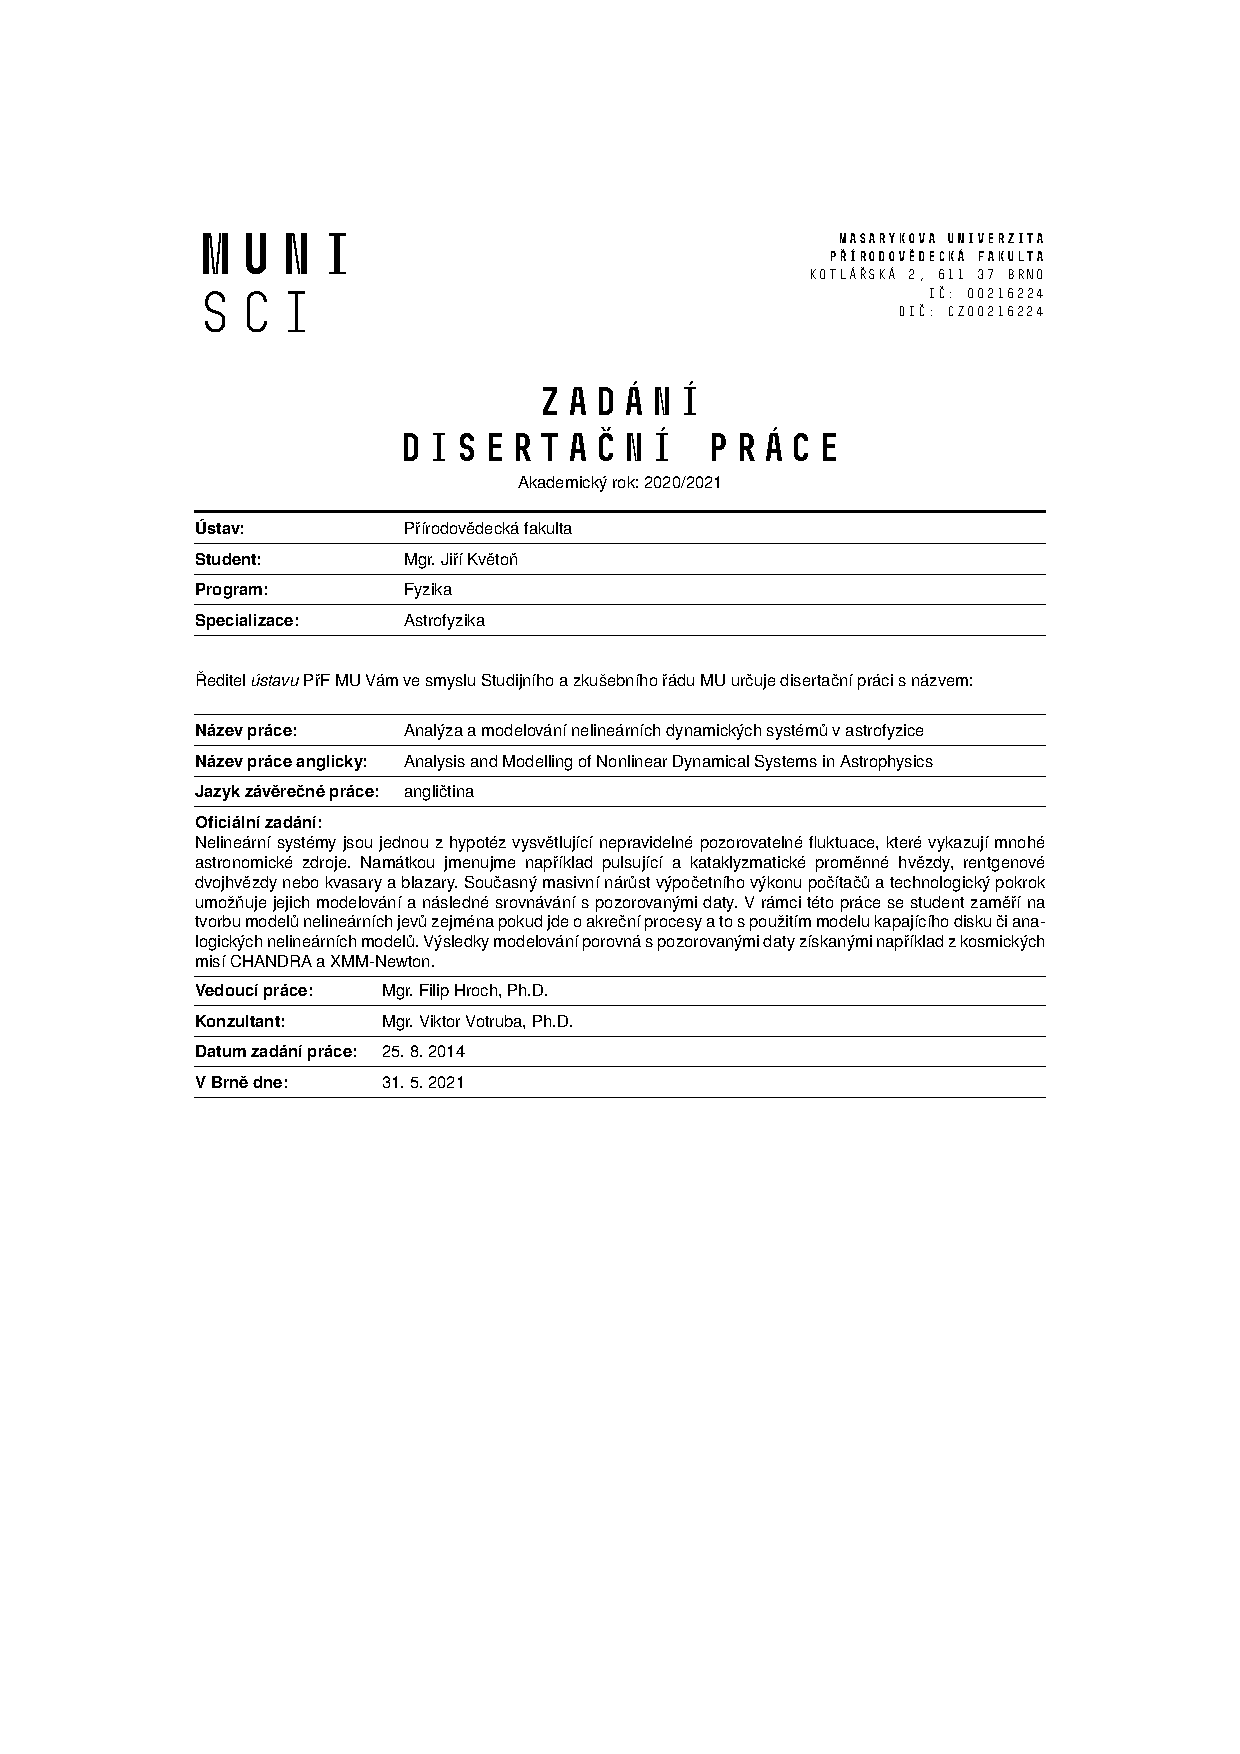
\includepdf[scale=0.85]{./misc/zadani.pdf}
    \blankpage

    \pagestyle{plain}

    % --
    % Bibliografický záznam
    % --
    %\phantomsection
    \bibinfoen

    %\phantomsection
    \bibinfocz

    % --
    % Abstrakt (CZ+EN)
    % --
    %\phantomsection
    \shortchapter{abstract}{./misc/abstract-en.tex}
    \blankpage

    %\phantomsection
    \shortchapter{abstrakt}{./misc/abstract-cz.tex}
    \blankpage

    % --
    % Poděkování
    % --
    %\phantomsection
    \shortchapter{acknowledgments}{./misc/acknowledgments.tex}
    \blankpage

    % --
    % Prohlášení
    % --
    %\phantomsection
    \declaration{./misc/declaration.tex}
    \blankpage

    % --
    % Copyright
    % --
    \copypage
    \blankpage

    % --
    % Obsah
    % --
    \content

    % Zapnout cislovani a vlastni styl hlavniho textu
    \pagestyle{mystyle}
    \pagenumbering{arabic}
    \setcounter{page}{1}    

    % 1. INTRODUCTION
    \chapter{INTRODUCTION}
\thispagestyle{empty}

\mquote{The Universe is under no obligation to make sense to you.}{Neil deGrasse Tyson}




    % 2. ACCRETION DISCS
    \chapter{ACCRETION DISKS}
    \label{chap:accretion_disks}
    The term \emph{accretion} comes from a Latin word \emph{accrescere} which literarily means \emph{become larger}, and in astrophysics, we refer exactly to that process. That is the \emph{coming together and cohesion of matter under the influence of gravity to form larger bodies} (citace). One could easily argue that it is one of the most fundamental processes in the universe. From the giant galaxies to the tiniest rocks floating around in the solar system. All the stars, planets, and all there is were smashed together by gravity at some point in the past. Atom by atom, piece by piece, to form larger and larger structures. Even the dinosaurs probably met their fate by a city-sized asteroid that accreted Earth some 65 million years ago. 

\section{Accreting systems}
    Accretion is not only the mass moving and colliding but also energy taking different forms in the process. Depending on the nature of the accreting system and its central object, radiation of various types is emitted by the accreted matter as it loses energy. Under certain conditions, the matter flow forms an accretion disk often closely confined to the orbital plane. If we sort accreting astrophysical systems based on their size, radiation power, and a few other characteristics, we can devise a crude classification of them. We will briefly describe the accreting system types in the following sections. 

\subsection{Active galactic nuclei (AGN) and Quasar}
    The high-luminosity region containing a supermassive black hole in most galaxies' centers is refered to as \emph{Active Galactic Nucleus}. The radiative power of the AGN is usually higher than that of the whole host galaxy, and the radiation characteristics indicate that stars are not the primary source of this radiation. Instead, mass accretion onto the central supermassive black hole is the more likely source of this excess non-stellar power output. 

    The main distinguishing characteristic of AGNs is whether they are \emph{radio loud} or \emph{radio quiet}, which depends on the existence of jets that are the source of radio radiation. By \emph{jets}, we mean relatively narrow streams of accreted mass ejected from the black hole in both directions, roughly colinear with its axis of rotation. These mass ejections can travel at relativistic speeds and reach thousands of light-years away from the source object. 

    Figure \ref{fig:centaurus_a_multiwave} shows the Centaurus A (NGC 5128) galaxy with a supermassive black hole in its center. This object is a typical \emph{radio loud} AGN. We can see both jets in the radio part of the spectrum and the accreted matter in other parts of the spectrum. For example, the galaxy,s dust core is most apparent in visible light.

    A particular sub-category of AGN is Quasars. The name \emph{Quasar} is a contraction of the phrase \emph{quasi-stellar radio source} because, in the 1950s, they were detected as radio sources of unknown physical characteristics and also in visible light as faint \emph{star-like} sources. However, they are nothing like stars. These highly luminous objects are observed to the highest values of redshift. The current record holder for the most distant Quasar is the J0313-1806 detected at redshift $z = 7.64$ by \cite{wang2021}. 

    Due to the extreme distance, it is impossible, at least with today's methods, to distinguish the active core (i.e., the supermassive black hole), whose mass can range from $10^6 M_{\odot}$ to $10^{9} M_{\odot}$. To this day, more than a million quasars have been discovered, with the closest known Markarian 231 (UGC 8058) at 581 million light-years away \cite{gaia2018}. 

    \begin{figure}
        \centering
        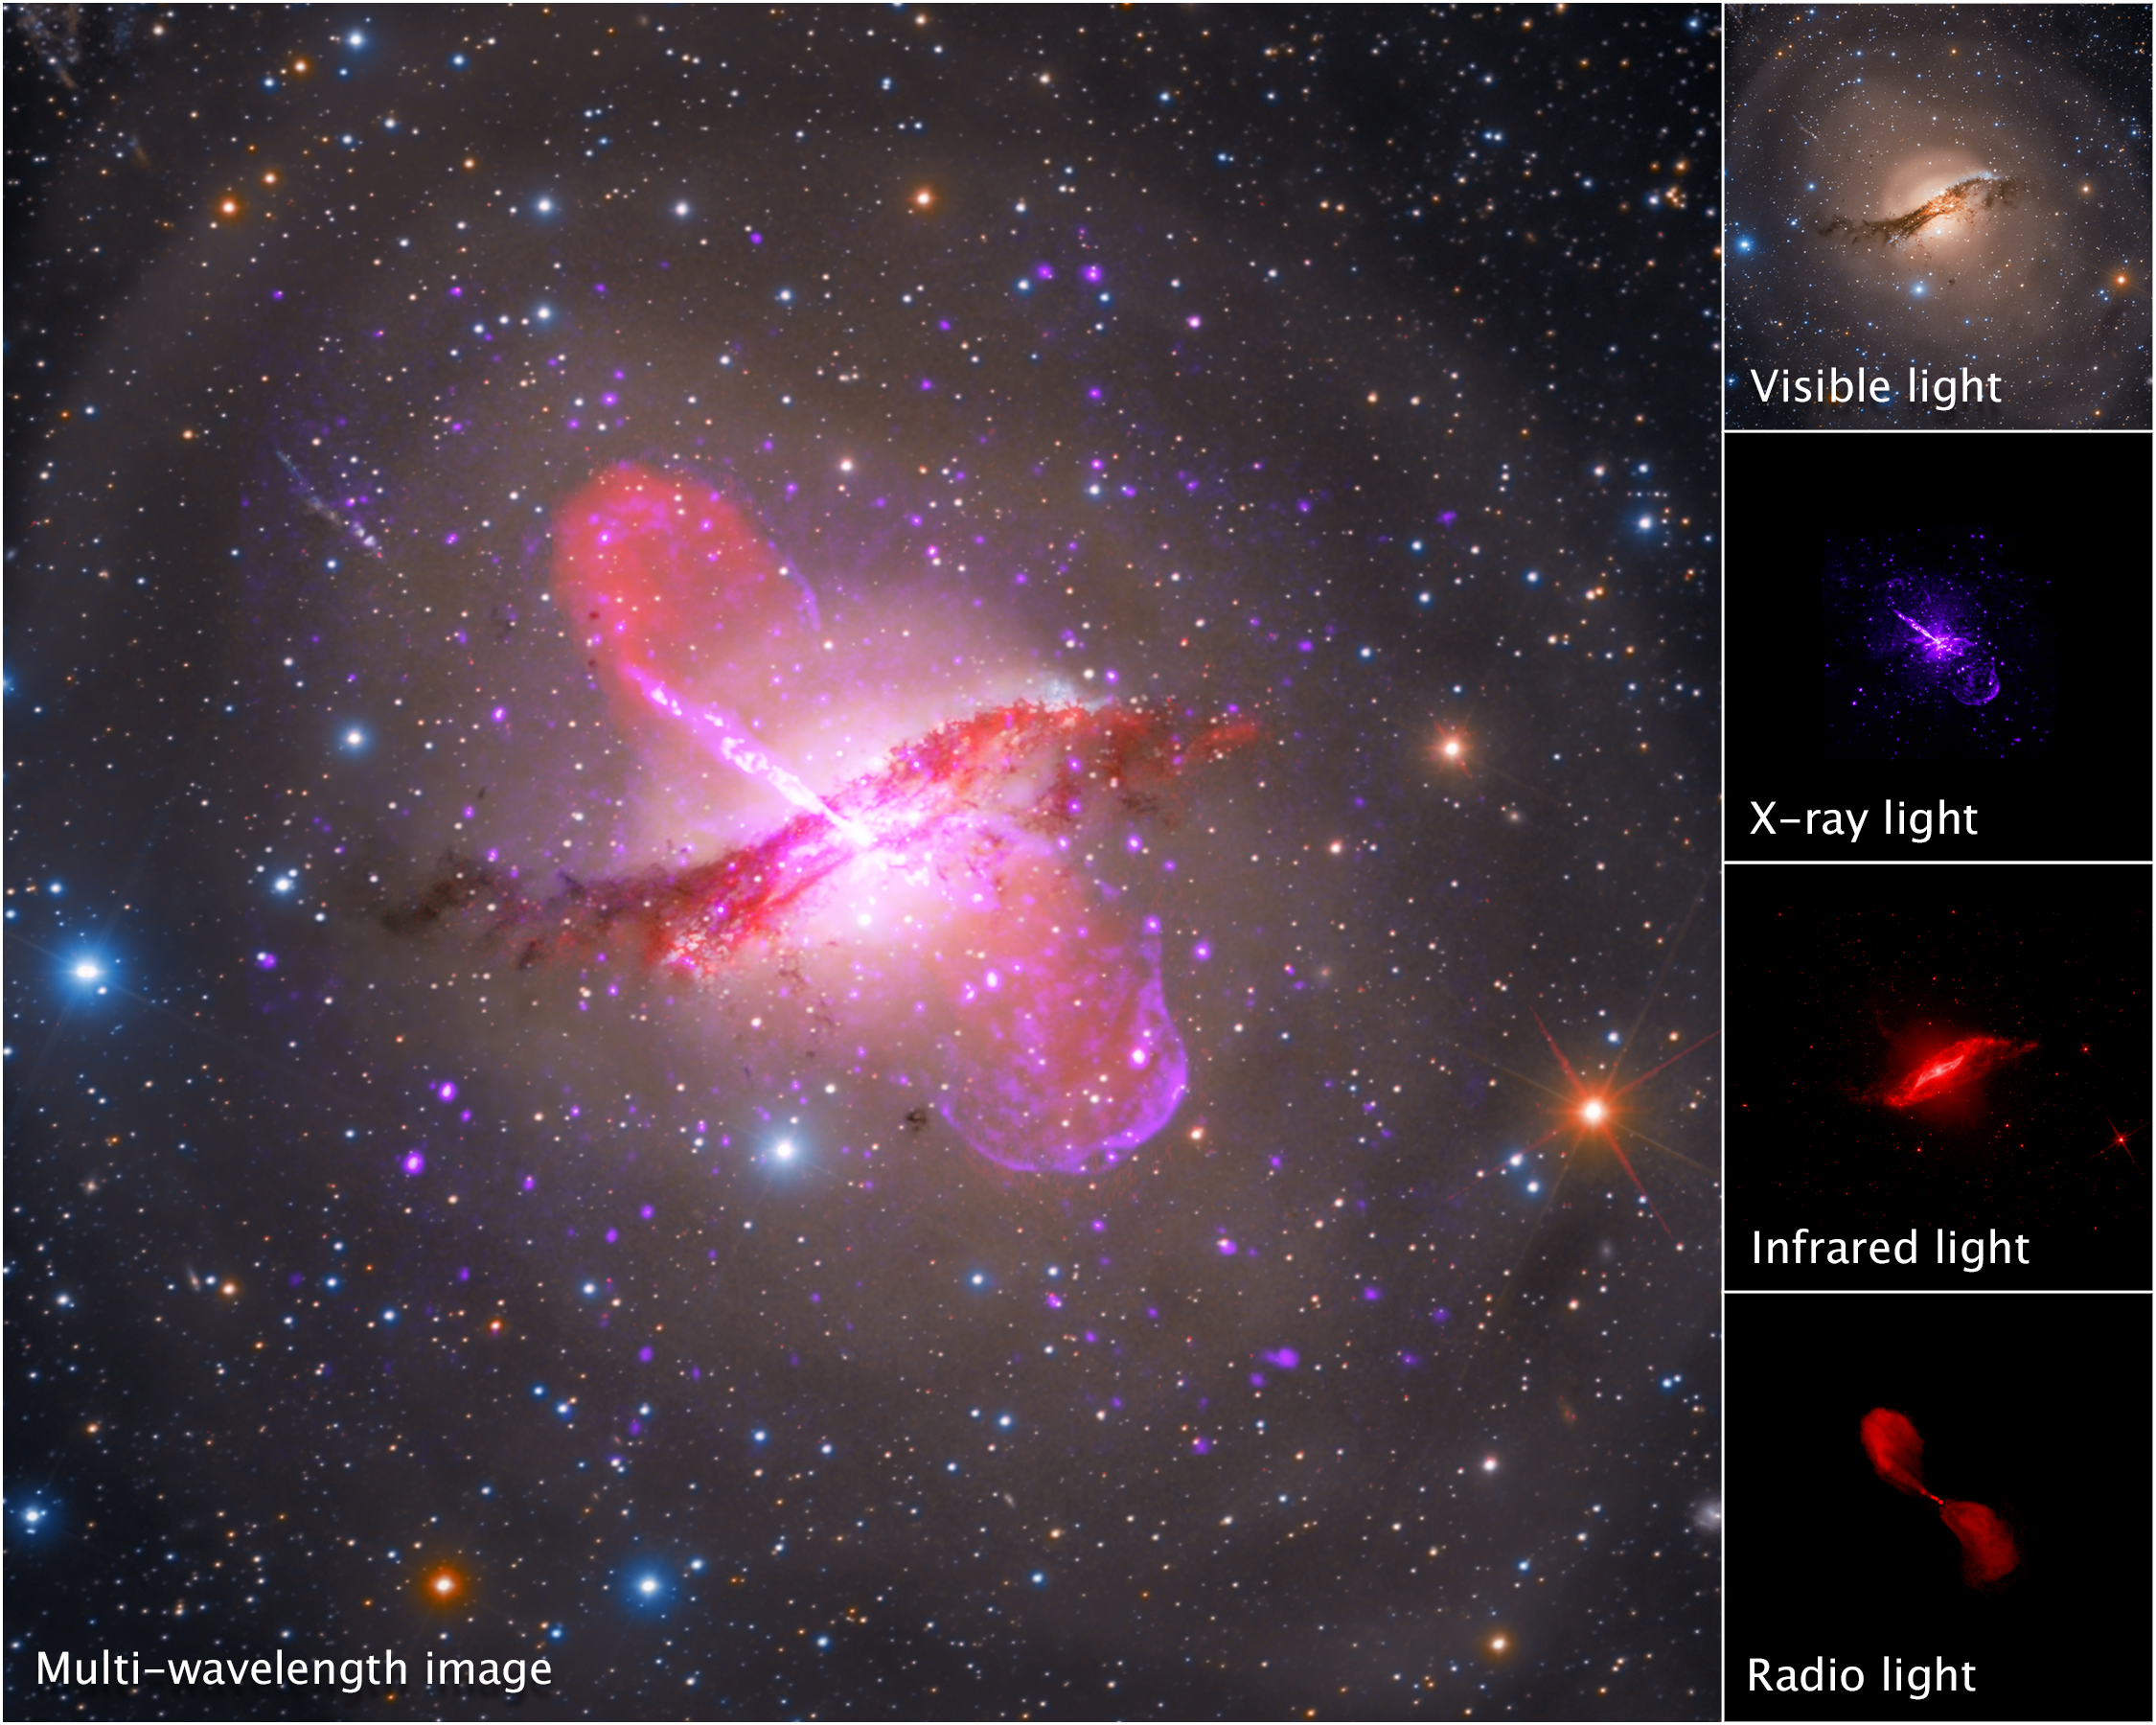
\includegraphics[width=\columnwidth]{img/multiwave_centaurus_a_agn.png}
        \caption{Multi-wavelength composition (left) and multiple narrow wavelength observations (right) of Centaurus A. Taken from \cite{nasa_img_centaurus_a}}
        \label{fig:centaurus_a_multiwave}
    \end{figure}

\subsection{X-ray binaries (XB)}
    The main sequence star in orbit around a neutron star (NSB - \emph{Neutron Star Binary}) or a black hole (BHB - \emph{Black Hole Binary}) is referred to as a \emph{X-ray binary} (XRB). The gravitational potential of these systems is strong enough that the accreted matter produces energy output up to the X-rays. Based on the mass of the primary component (i.e., the accretor), this class of binary stars is also usually split between \emph{Low-mass X-ray binary} (LXRB) and \emph{High-mass X-ray binary} (HXRB). 

    Most XRB objects go through periods of high activity when they emit twin jets at relativistic speed, not that dissimilar to AGN but at a smaller scale, and then a period of relative quiescence.

    In the special case, when the accretor is the strongly magnetized young neutron star, the accretion disk is truncated by its magnetic field or not present at all, and the matter transfers onto the neutron star by \emph{column accretion}.

    %% TODO: Muj Cygnus X-1 pro demonstraci

\subsection{Young stellar objects (YSO)}
    When a proto-star is formed from a collapsing molecular cloud, the gas and solid particles envelope forms a rotating protoplanetary accretion disk. Instabilities and self-gravity in the disk's body eventually lead to planets and other smaller objects forming. The proto-star is only detectable in infrared due to the relatively dense surrounding matter that obscures it. 

    The YSO classification consists of five classes (0-IV) based on the infrared and visible spectral energy distribution. Class 0 is a collapsing molecular cloud. Classes I to III are YSO with a formed proto-planetary disk in various stages of evolution, and lastly, class IV refers to a fully formed zero-aged star. 

    \begin{figure}[h]
        \centering
        \includegraphics[width=\columnwidth]{img/jwst_protostar_l1527.png}
        \caption{Proto-star L1527 captured by Near-Infrared-Camera (NIRCam) onboard the JWST. Taken from \cite{nasa_img_l1527}}
        \label{fig:jwst_protostar_l1527}
    \end{figure}


    As a side note, the \emph{James Webb Space Telescope} (JWST) was released only a year ago, on December 25, 2021. It is equipped with multiple near-infrared and infrared instruments, so it is literarily able to see through the clouds of such objects and uncover the stars being born. Due to JWST's observational capabilities and the sheer size of its primary mirror, we have something to look for in this particular field of astrophysical research. The first glimpses of JWST observations demonstrate the spectacular Figure \ref{fig:jwst_protostar_l1527}, showing the proto-star L1527 captured by the Near-Infrared-Camera (NIRCam). 

\subsection{Gamma-ray bursts (GRB)}
    Highly energetic, collimated flashes of $\gamma$-rays that can last tens of milliseconds up to several hours are called \emph{Gamme-ray burts} (GRB). These are considered the most energetic events in the observable universe. In addition, GRBs are accompanied by simultaneous radiation on longer wavelengths (e.g., X-ray) and a follow-up slowly fading afterglow that may be observable for up to several years. 

    It is theorized that the possible origin of GRBs may be a compact object merger or a \emph{collapsar} (i.e., the failed supernovae). The observations indicate the formation of a black hole with an accretion disk surrounding it and a high mass accretion rate \cite{piran2005}.

    One of the brightest detected GRB 221009A (Swift J1913.1+1946) was detected very recently on October 9, 2022, by the orbital \emph{Neil Gehrels Swift Observatory} \cite{grb_221009a}. It is also one of the closest observed GRBs. 

    %% TODO: obrazek GRBu??? -> spis neni potreba

\subsection{Cataclysmic variables (CV)}
    We are particularly interested in CVs in this study because our modeling efforts in the latter chapters focus on generic CV systems. Unlike the LMXB or HMXB, where the primary component is either a black hole or neutron star, the accretor in CV is a White Dwarf (WD), and its companion is a late-type star. Due to its nature, this system has a relatively weaker gravitational potential; therefore, its radiation energy output is lower than that of the XRB and is comparable in size to planetary or Earth-Moon-like systems. 

    The primary WD is a stellar core remnant composed of very dense electron-degenerate gas, and its size can be approximated by the \emph{mass-radius ratio} \cite{shapiro1983}

    \begin{equation}
        r_{\textrm{in}} \sim M^{-1/3}_{\textrm{p}},
        \label{eq:mass_radius_ratio}
    \end{equation}

    where $M^{-1/3}_{\textrm{p}}$ represents the WD mass and $r_{in}$ its radius, which also corresponds to the inner boundary layer radius of the accretion disk.

    The secondary component star fills its Roche lobe, and the overflowing matter falls onto the WD through the Langrangian point $L_1$ \cite{warner1995}. If the WD is not magnetized or weakly magnetized, the gas stream forms an accretion disk around the WD that eventually reaches its surface. In the case of strongly magnetized WD, the accretion disk is truncated or non-existent, and the magnetic field lines direct the accretion flow (citace). 

    Another important parameter of the CV binary system is its component separation distance, closely related to individual component masses. It determines the accretion disk size because the gravitational potential constrains its outer edge. The outer disk radius is calculated

    %% TODO: Citace vypoctu? Podrobnejsi vyjadreni

    \begin{equation}
        r_{out} = d \left[ \frac{M_{\textrm{s}}}{3(M_{\textrm{p}}+M_{\textrm{s}})} \right]^{1/3},
        \label{eq:disk_outher_radius}
    \end{equation}

    where $M_{\textrm{s}}$ represents the secondary component's mass and $d$ is the distance between the components. Equations \eqref{eq:mass_radius_ratio} and \eqref{eq:disk_outher_radius} give us the inner and outer constraints to define the geometry of the model, which we will define in the latter chapters of this study.   

\section{Accretion disks models}
    For the accreting matter that dissipates energy and is not supported by internal pressure, the matter will form an accretion disk, which is its minimal energy configuration. The falling matter must lose angular momentum to reach the central object. This process is done through a \emph{viscous disipation} that is key in transporting the angular momentum outward and heats the disk. The nature and magnitude of the viscous processes are the questions of accretion disk modeling because they are the critical factor determining the disk size, shape, optical dept, and radiation properties. It still needs to be better understood in the case of accretion disk matter flow because the disk's body consists of a sheering, radiative, and supersonic medium with a high Reynold's number \cite{pringle1981}, and that is quite a challenging problem to model. 

    Then there is a question of magnetic fields. The central object (i.e., WD or NS) may or may not be magnetized. Some objects rotate very fast. For example, NS rotation periods range from a couple of milliseconds to tens of seconds. The temperature and composition of the material inflow can widely differ depending on the characteristics of the secondary object. All those factors add up and create a complex non-linear accretion environment. Therefore, when modeling such a complex and dynamic astrophysical system, we are inevitably forced to make some simplifications, neglections, and approximations. 

    In many cases, the accretion disk is closely confined to an orbital plane, so in the first approximation, we may regard the disk's matter flow as two-dimensional, ad we call this the \emph{thin disc approximation}. This simple yet very effective simplification enables the creation of a very elaborate accretion model's theory, but with reduced complexity, \cite{acpow}.

\subsection{Sub-Eddington accretion disks}
    The standard vertically \emph{thin} accretion disk is formed under the conditions of sub-Eddington accretion rate and very high opacity. The Eddington limit is the maximum luminosity of a radiating body in hydrostatic equilibrium, which means the radiation and gravitational forces acting in opposite directions are in balance. The accreting matter follows very tight spiraling orbits that are almost Keplerian. Moreover, thin disks have a relatively high luminosity with spectral energy distribution closely resembling a \emph{black body} radiation. Thin disks theory was devised almost independently by \cite{lyndenbell1974}, \cite{pringle1981}. Under the umbrella of \emph{standard thin disks} is also the Shakura-Sunyaev $\alpha$-disc model, which is described more closely in Section \ref{sec:alpha_model_definition}. This model is particularly interesting to us because part of our simulation efforts in the latter chapters is focused on the $\alpha$ parameter modeling.

    In the case of the central object in the thin disc system being a black hole, the models need to deal with relativistic effects in its proximity. Researchers D. N. Page and K. S. Thorne provided such a theory in \cite{page1974}, which was later used by \cite{luminet1979} and \cite{marck1996} to generate synthetic images of Keplerian disk around a black hole distorted by intense gravitational lensing. Figure \ref{fig:bh_warped} shows a more recent simulation example of such a synthetic image. 

    \begin{figure}[h]
        \centering
        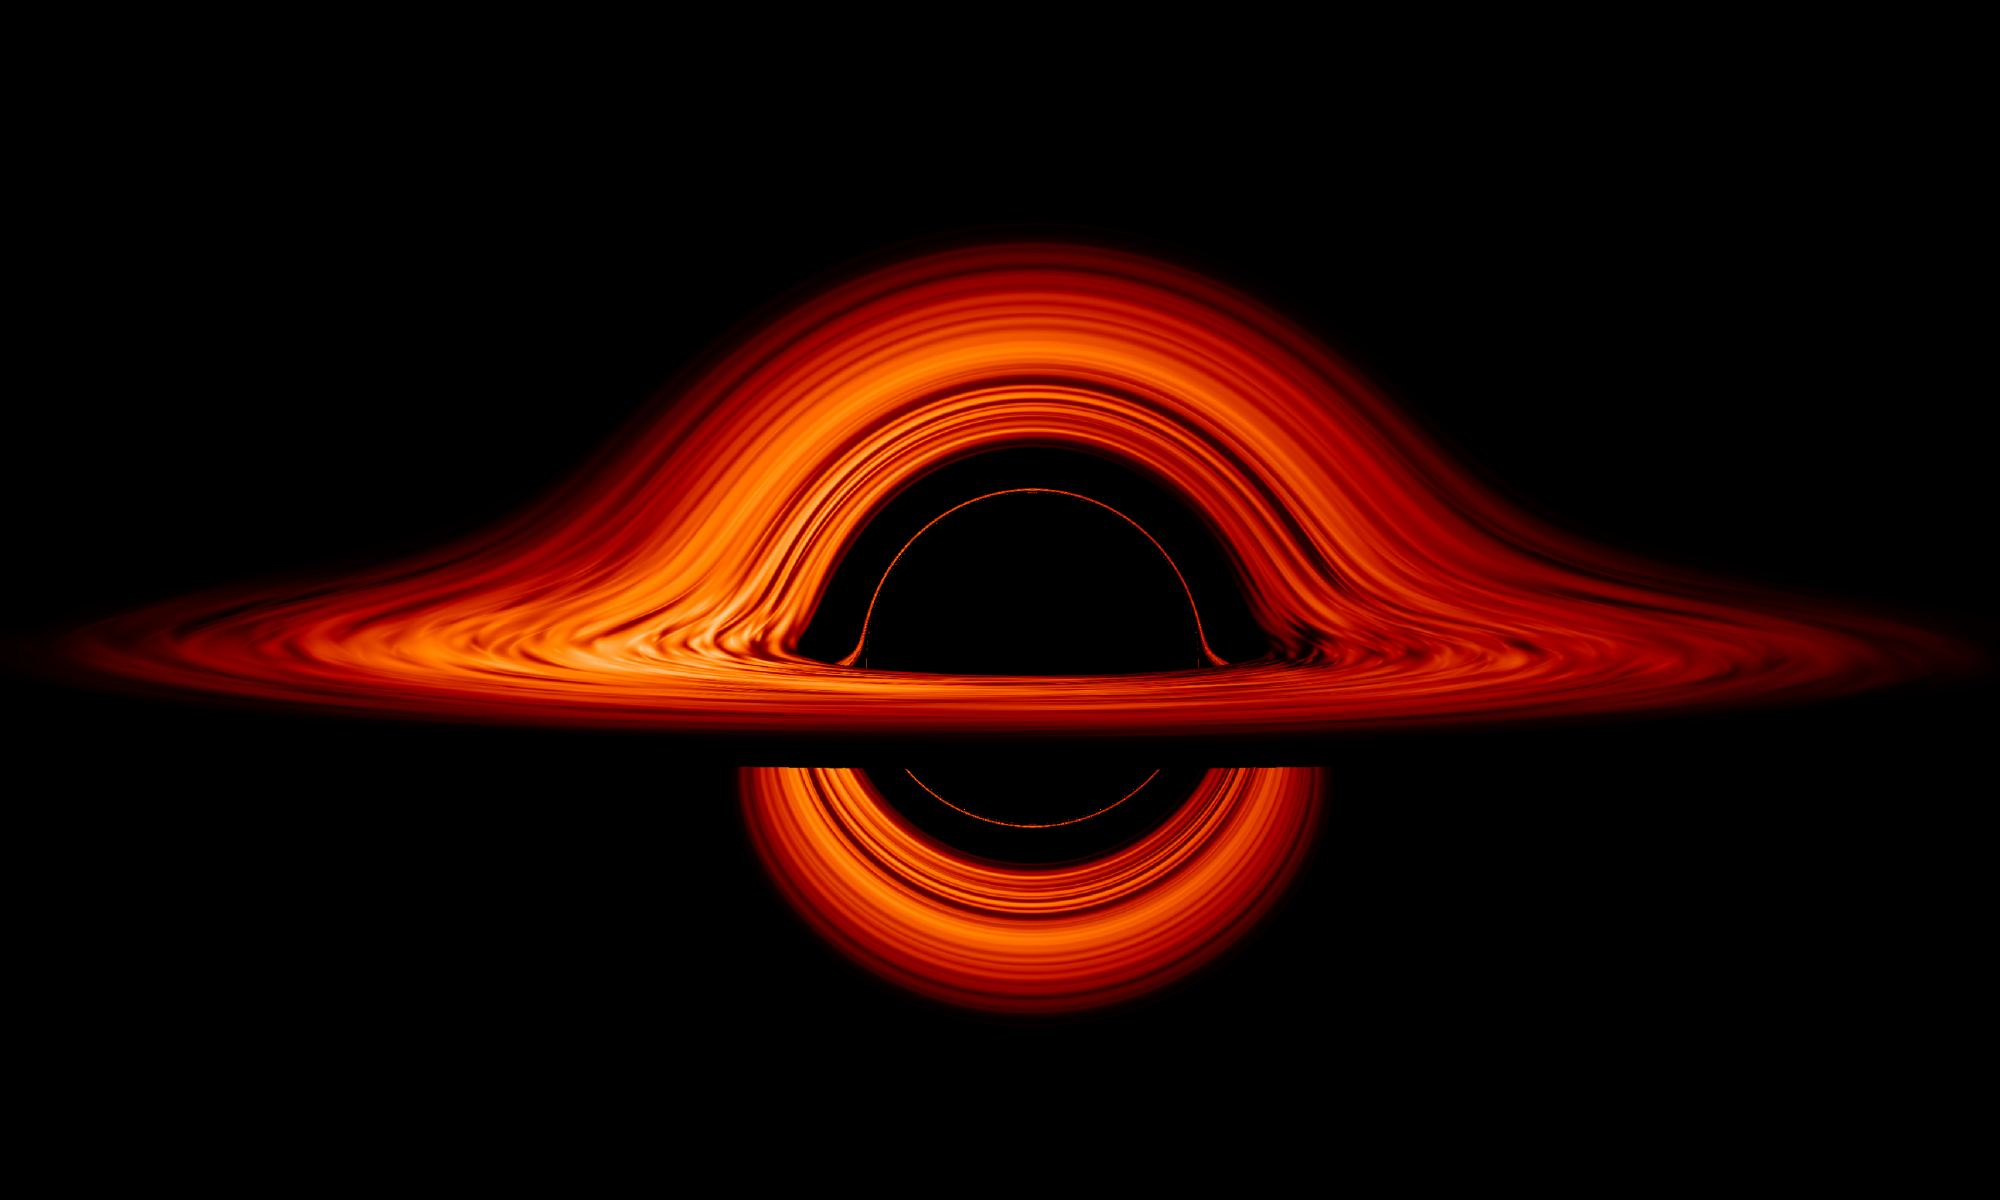
\includegraphics[width=1.0\columnwidth]{img/bh_warped.jpg}
        \caption{Visualization of a black hole accretion disk. The observer's image is warped by extreme gravitational lensing and highly depends on the observer's inclination. Taken from \cite{nasa_img_bh_warped}}
        \label{fig:bh_warped}
    \end{figure}

    As a side note, these simulated images found their way even to a broader audience through pop-cultural references. Professor Thorne himself worked as a science advisor for Christopher Nolan's 2014 movie Interstellar, in which very accurate VFX renders of a supermassive black hole with an accretion disk were used. 

    The other type of sub-Eddington disk that, forms when the opacity is very low, is called ADAF (\emph{Advection-Dominated Accretion Flows}), and it was predicted by \cite{ichimaru1977}. ADAFs are radiatively very inefficient, because the cooling is done dominantly by advection (i.e., heat capture in the matter) and not by radiation. Therefore they are very hot, geometrically extended and more similar in shape tho a sphere than a flat disk \cite{acpow}.

\subsection{Super-Eddington accretion disks}
    Doplnit!!!

    % TODO: doplnit Super-Eddington disky

\subsection[Shakura-Sunyaev $\alpha$-Disc model]{Shakura-Sunyaev $\alpha$-disc}
    \label{sec:alpha_model_definition}
    In 1973, N. I. Shakura and R. Sunyaev proposed an accretion disk model whose source of increased viscosity are the turbulent flow patterns in the disk's body \cite{shakura1973}. This model applies if the modeled system is a \emph{thin disk}, and because of that, it is considered that all material in the disk's body is near its surface, allowing the thermal emission to escape freely. Therefore, self-absorption processes are insignificant. 

    Utilizing equations of hydrostatic equilibrium and Kramer's opacity law on the two-dimensional disk, we can devise a set of equations that describe the local disk structure \cite{acpow}

    \begin{align}
    \begin{split}
        \rho &= \Sigma / H, \\
        H &= c_{\mathrm{s}} R^{3/2} / (GM)^{1/2}, \\
        c_{\mathrm{s}}^2 &= P / \rho, \\
        P &= \frac{\rho k T_{\mathrm{c}}}{\mu m_p} + \frac{4 \sigma}{3 c}T_c^4, \\
        \frac{a \sigma T_{\mathrm{c}}^4}{3 \tau} &= \frac{3GM\dot{M}}{8 \pi R^3}, \\
        \tau &= \Sigma \kappa_{\mathrm{R}}(\rho, T_{\mathrm{c}}) = \tau(\Sigma, \rho, T_{\mathrm{c}}), \\
        \nu \Sigma &= \frac{\dot{M}}{3 \pi} \left[ 1 - \left( \frac{R_*}{R} \right)^{1/2} \right], \\
        \nu &= \nu(\rho, T_{\mathrm{c}}, \Sigma, \alpha, ...).
    \end{split}
    \label{eq:alpha_model_prescription}
    \end{align}

    The set of equations \eqref{eq:alpha_model_prescription} contains eight unknowns: density $\rho$ and temperature $T_{\mathrm{c}}$ of disk's mid-plane, scale height $H$ of the disk, the speed of sound in the medium $c_s$, the sum of gas and radiation pressure $P$, area density $\Sigma$, optical depth $\tau$, and viscosity $\nu$. These unknowns are solved as functions of: accretion rate $\dot{M}$, the central object's mass $M$, the radius of a specific point in the disk $R$, and free parameter $\alpha$. Moreover, $R_*$ represents the radius where angular momentum stops being transported outwards. Assuming that the values $\rho$ and $T_{\mathrm{c}}$ enable the approximation of Rosseland mean opacity using Kramer's law

    \begin{equation}
        \kappa_{\mathrm{R}} = 5 \cdot 10^{24} \rho T_{\mathrm{c}}^{-7/2} \si{\cm^2 \gram^{-1}},
    \end{equation}


    the viscosity of the disk's medium is estimated

    \begin{equation}
        \nu = \alpha c_{\mathrm{s}} H,
    \end{equation}

    where $c_{\mathrm{s}}$ represents the speed of sound in the medium. $H$ represents the scale height of the disk limiting the subsonic turbulent eddies size. The free parameter $\alpha$ ranges between zero (no accretion) and approximately one. Solving the equations \eqref{eq:alpha_model_prescription} with the assumption $\mu = 0.615$ (fully ionized gases), we get a set of relations representing the Shakura-Sunyaev $\alpha$-disc solution \cite{acpow}  

    \begin{align}
    \begin{split}
    \Sigma &= 5.2 \alpha^{-4/5} \dot{M}^{7/10}_{16} m^{1/4}_1 R^{-3/4}_{10} f^{14/5}\ \mathrm{g\ cm^{-2}}, \\
    H &= 1.7 \times 10^8 \alpha^{-1/10} \dot{M}^{3/20}_{16} m^{-3/8}_1 R^{9/8}_{10} f^{3/5}\ \mathrm{cm}, \\
    \rho &= 3.1 \times 10^{-8} \alpha^{-7/10} \dot{M}^{11/20}_{16} m^{5/8}_1 R^{-15/8}_{10} f^{11/5}\ \mathrm{g\ cm^{-3}}, \\
    T_{\mathrm{c}} &= 1.4 \times 10^4 \alpha^{-1/5} \dot{M}^{3/10}_{16} m^{1/4}_1 R^{-3/4}_{10} f^{6/5}\ \mathrm{K}, \\
    \tau &= 190 \alpha^{-4/5} \dot{M}^{1/5}_{16} f^{4/5}, \\
    \nu	&= 1.8 \times 10^{14} \alpha^{4/5} \dot{M}^{3/10}_{16} m^{3/4}_1 R^{3/4}_{10} f^{6/5}\ \mathrm{cm^2\ s^{-1}},  \\
    v_{\mathrm{R}}	&= 2.7 \times 10^{14} \alpha^{4/5} \dot{M}^{3/10}_{16} m^{-1/4}_1 R^{-1/4}_{10} f^{-14/15}\ \mathrm{cm\ s^{-1}},  \\
    \mathrm{with}\ f &= \left[ 1 - \left( \frac{R_*}{R} \right)^{1/2} \right]^{1/4}, \\
    \end{split}
    \label{eq:alpha_model_solution}
    \end{align}

    where $f$ represents the boundary layer function. $\dot{M}_{16}$, $R_{10}$, and $m_1$ are transformed to be represented in typical sizes of disk quantities

    \begin{align}
    \begin{split}
        \dot{M}_{16} &= \dot{M} / 10^{16} \si{\gram \second^{-1}}, \\
        R_{10} &= R / (10^{10} \si{cm}), \\
        m_1 &= M / M_{\odot}.
    \end{split} 
    \end{align}

    Figure \ref{fig:plot_alpha_H_T} shows $T_{\mathrm{c}}$ and $H$ solution examples using different values of free parameter $\alpha$ for the same accretion disk system.

    \begin{figure}[H]
        \centering
        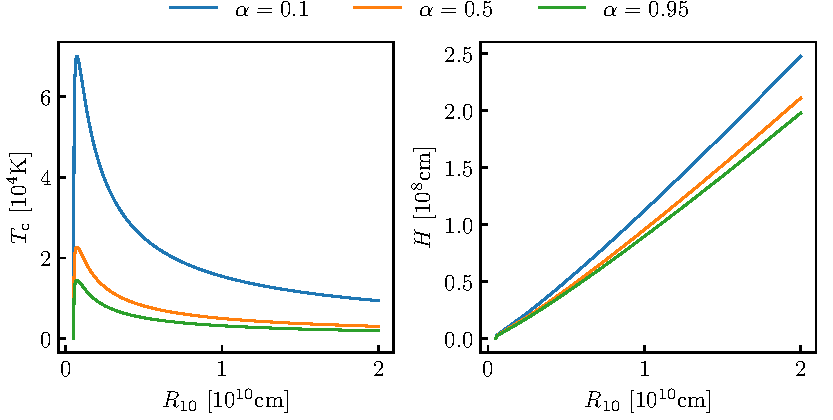
\includegraphics[scale=1.0]{img/plot_alpha_H_T.pdf}
        \caption{$\alpha$-disk model solution examples. Chosen central object's mass is $m_1 = 0.8$. Mid-plane temperatue $T_{\mathrm{c}}$ solution (left) and scale height $H$ (right).}
        \label{fig:plot_alpha_H_T}
    \end{figure}

    
    % 3. CATACLYSMIC VARIABLES
    \chapter{CATACLYSMIC VARIABLES}
\thispagestyle{empty}


    % 4. FLICKERING PHENOMENON
    \chapter{FLICKERING PHENOMENON}
\thispagestyle{empty}


    % 5. SIMILARITY OF NON-LINEAR SYSTEMS
    \chapter{SIMILARITY OF NON-LINEAR SYSTEMS}
\label{chap:similary_of_nonlinear_systems}
\thispagestyle{empty}



    % 6. DRIPPING FAUCET
    \chapter{DRIPPING FAUCET}




\section{Fluid dynamical model (FDM)}
\section{Mass-spring model (MSM)} \label{section:msm}

\thispagestyle{empty}


    % 7. DRIPPING HANDRAIL MODELS
    \chapter{DRIPPING HANDRAIL MODELS}
\thispagestyle{empty}


    % 8. MDH - MODEL DEFINITION 
    \chapter{MDH - MODEL}
\thispagestyle{empty}

\mquote{The universe doesn't care if we understand it.}{Honey Badger Ph.D.}

Accretion disc model developed for the purpose of this study is composed of $n$ times $m$ individual cells arranged in concentric circular grid, where $n$ is the number of concentric layers and $m$ number of cells in its layers.

Each cell holds a set of parameters and its behaviour is governed by set of ordinary differential equations derived from MSMM \footnote{Defined in section \ref{section:msm}.}, so fundamentally every cell is its own \emph{dripping faucet}. Layers move in the same direction\footnote{Direction is arbitrary and a matter of perspective (i.e. top vs. bottom view).} with Keplerian orbital velocities relative to the outermost layer, which move by exactly one cell angular length in one simulation step. In every simulation step, there is a predefined constant mass influx into the outermost layer. This influx could come from specific azimuth or it could be distributed in some probabilistic manner from a wider range of angels.

As the simulation progresses, the mass is distributed in tangential direction by the orbital movement of layers and in radial direction by overflow from individual cells. This radial mass transfer is unidirectional towards the grid center and is triggered by a critical condition of MSMM in specific cells. 

Cell parameters and radial mass overflow are logged separately and later used to compute the radiative output, which is strongly dependent on radial mass transfer through changes in cell temperature and energy losses in gravitational potential of the imagined central body. 

Based on its characteristics, this model is called a \emph{Multilayer Dripping Handrail} and hereinafter it shall be referenced as MDH.

\section{MDH grid structure}

The cells are arranged in concentric circular grid of $n$ layers and $m$ cells in each layer. Layers are denoted by $i \in [0, n-1]$, with the outermost layer having the index $i = 0$. Individual cells in each layer are denoted by $j \in [0, m-1]$\footnote{Direction of $j$ index iteration is arbitrary and depends on implementation.}. Figure \ref{fig:grid_states} shows simplified representation of this concentric simulation grid in a) its initial state and b) in shifted state after arbitrary number of simulation steps. 

\begin{figure}
\centering
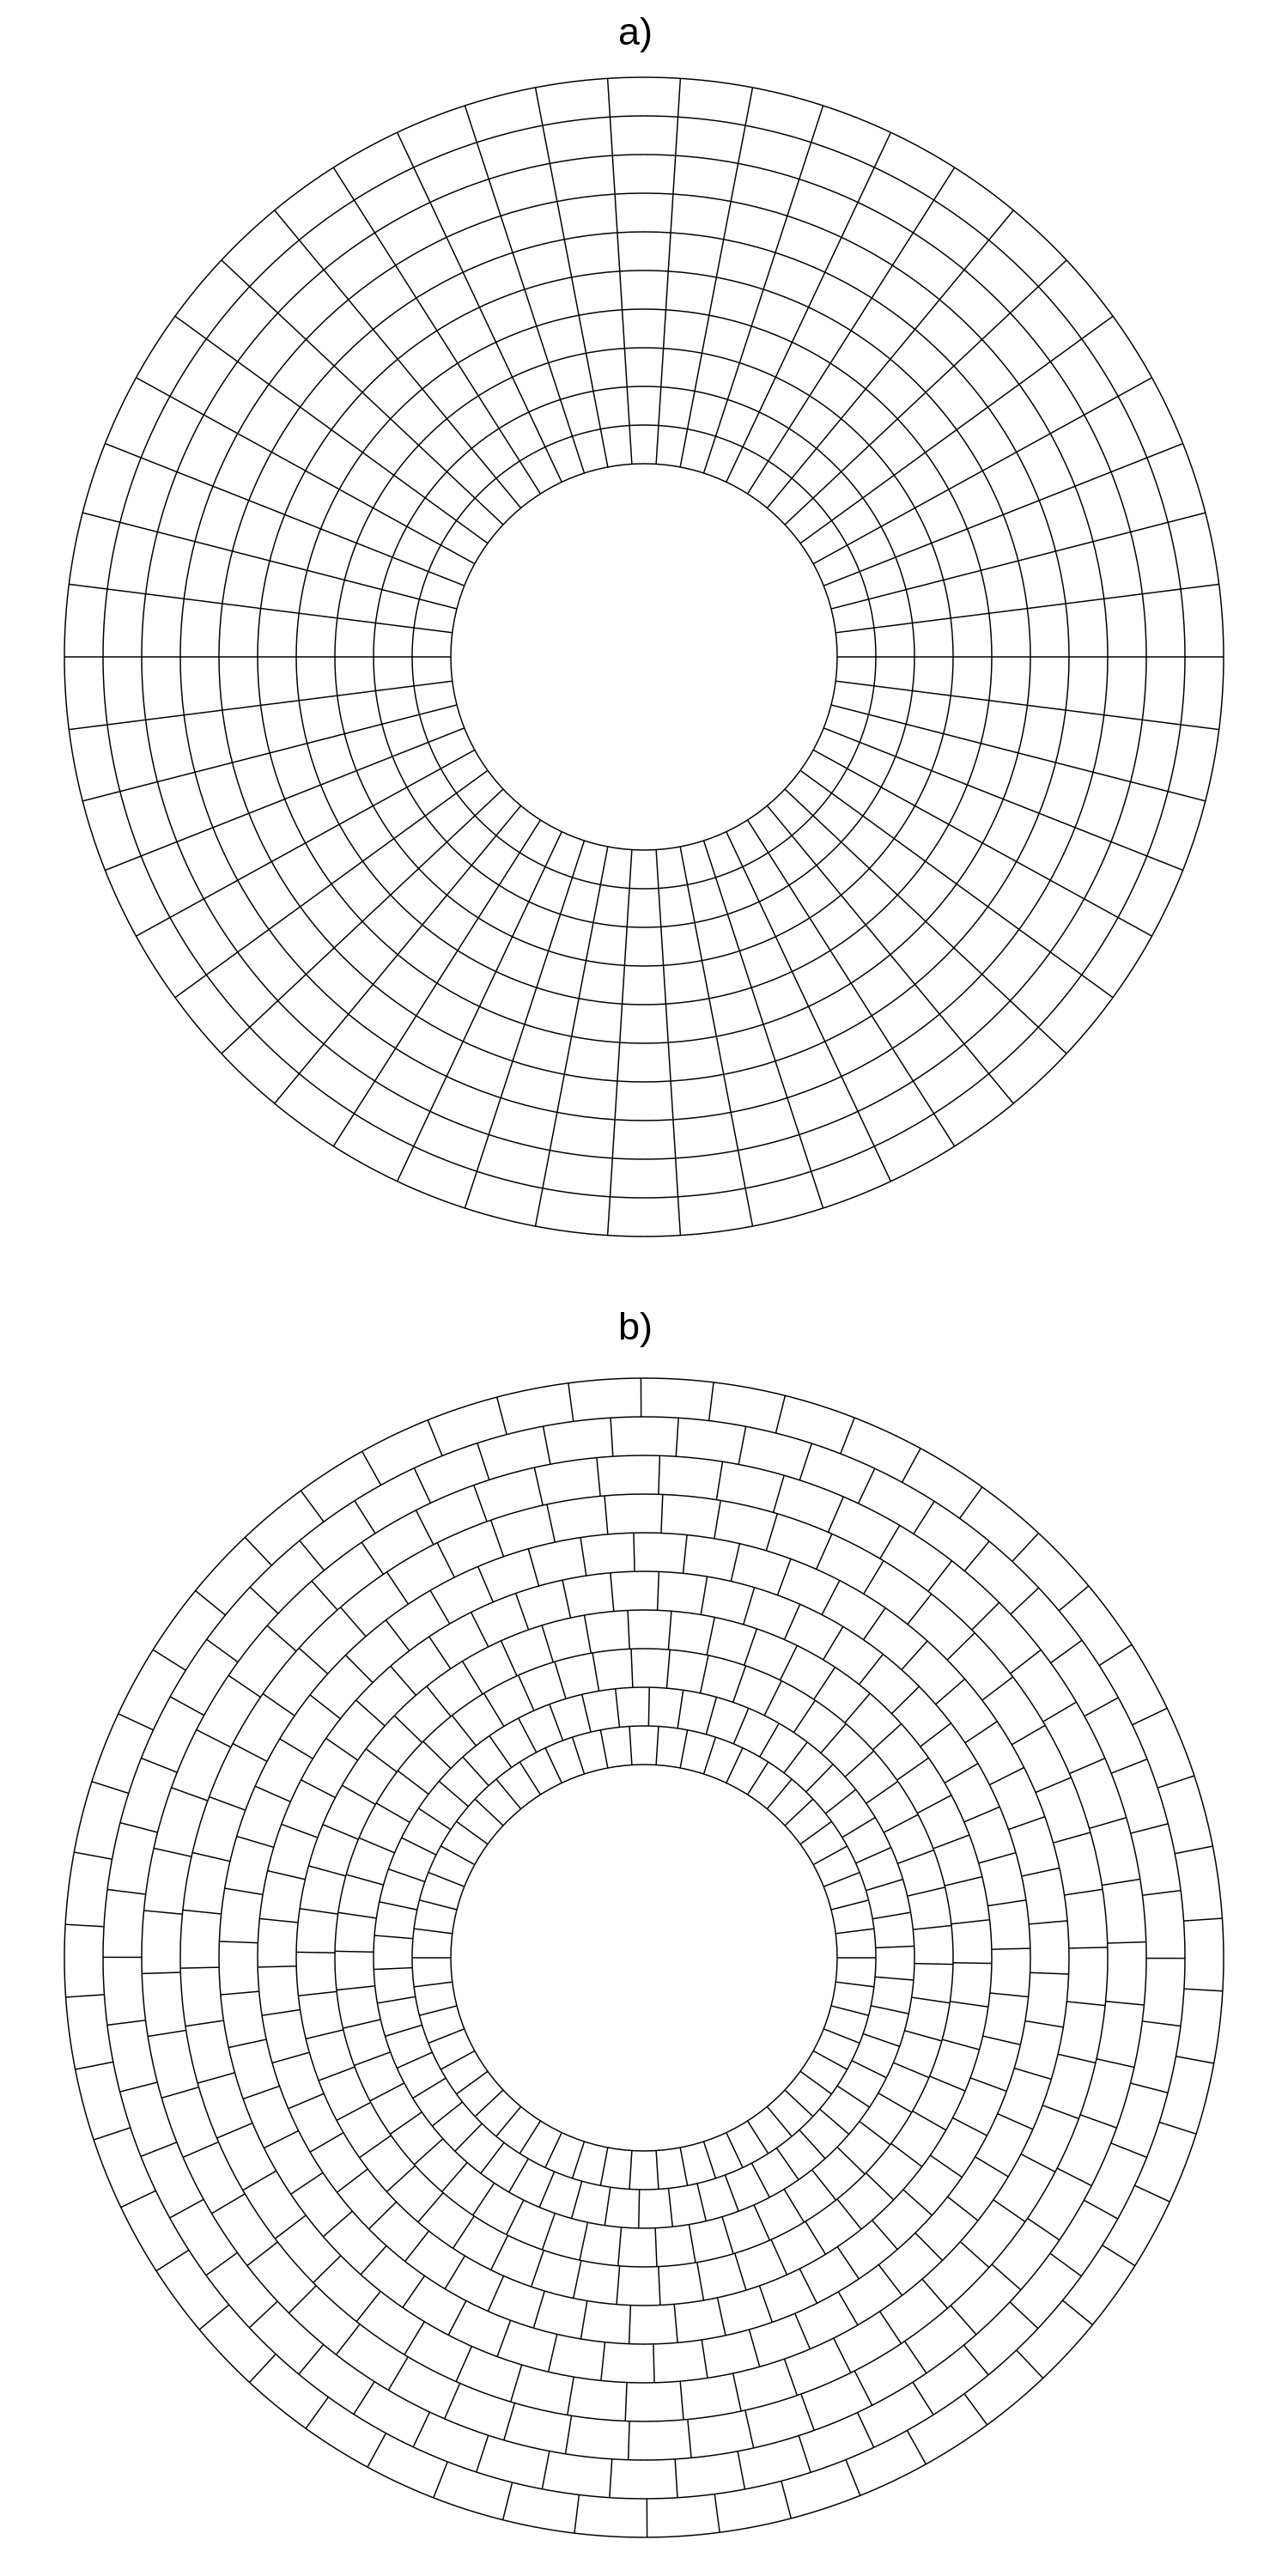
\includegraphics[width=0.75\columnwidth]{img/grid_states.png}
\caption{Simulation grid states: a) Initial unshifted state b) Shifted state after arbitrary number of simulation steps}
\label{fig:grid_states}
\end{figure}

Whole simulation grid acts like a cellular automaton (CA). Cellular automata models usually implement some kind of simple condition or set of conditions (e.g. Conway's game of life, see \cite{gardner1970}), to decide simulation development for the next step. In the case of model created by \cite{yonehara1997}, there is a simple mass limit condition to trigger the radial mass transfer. MDH takes this concept further and implements the condition as critical value of \emph{spring elongation} $z$ of MSMM, which is the solution of its ODE system solved in every simulation step. 

\section{Cell definition}
Individual cells are defined by a set of parameters. These parameters are listed in table \ref{table:mdh_cell_parameters} and following sections discuss some of them in detail.

\begin{table}[h]
\begin{center}
\begin{tabular}{r|l}
$i$			& Layer index \\
$j$			& Cell index \\
$r$			& Orbital radius \\
$\theta$	& Orbital azimuth \\ 
$f_g$		& Gravitational acceleration relative to outermost layer \\
$z$			& MSMM \emph{spring elongation}  \\
$v$			& MSMM \emph{velocity} \\
$m$			& Mass contained within the cell \\
$\Delta m$ 	& Mass change since previous step \\
$\gamma$		& Constant MSMM dampening parameter \\
$k$			& MSMM \emph{spring stiffness} \\
$T$			& Cell temperature
\end{tabular}
\caption{MDH model cell parameters}
\label{table:mdh_cell_parameters}
\end{center}
\end{table}

\subsection{MDH model geometry}
Position and size of specific cell in MDH model is derived from real world geometry of modelled accretion disc system. Parameters in question, are the orbital radius $r$ and orbital azimuth $\theta$. To define the orbital radius $r$, first the inner $r_{in}$ and outer $r_{out}$ radii of the accretion disc must be defined. The modelled system is considered to be a typical CV star\footnote{MDH can be modified to be applicable to other types of accreting systems.}, therefore in the first approximation $r_{in}$, that defines the boundary layer between accretion disc and central body, is set to be equal to the radius of the white dwarf. Using the \emph{White Dwarf Mass-Radius Relationship} it can be estimated, that radius is inversely proportional to the cube root of white dwarfs mass (citace!!):

\begin{equation}
    r_{in} \sim M_p^{-1/3},
\end{equation}

\begin{equation}
	r_{in} = 2 \cdot 10^{4} \left(\frac{\beta}{0.5}\right)^{5/3} \left(\frac{M_p}{M_{\odot}}\right)^{-1/3},
\end{equation}

where $M_p$ represents mass of the white dwarf and $\beta$ is ??? . Outer radius $r_{out}$ represents the outer edge of accretion disc, that is constrained by the Roche potential (citace!!!). Outer radius $r_{out}$ is then calculated as:

\begin{equation}
    r_{out} = d \cdot \frac{M_{s}}{3 \cdot (M_p+M_{s})^{1/3}},
\end{equation}

where $d$ represents the distance between binary system components and $M_s$ represents mass of the secondary donor star. Space between $r_{in}$ and $r_{out}$ is discretize into regularly spaced intervals according to chosen radial dimension $n$:

\begin{equation} \label{eq:cell_radius}
    r_i = r_{in} + (n - i - 1) \cdot \frac{r_{out} - r_{in}}{n - 1},
\end{equation}

\subsection{Azimuth and angular velocity profile}
Accretion disc layers (i.e. rings) are divided into equally spaced $m$ number of cells. Angular position is expressed by its orbital azimuth $\theta \in [0, 2\pi]$. Because orbits are considered to be Keplerian, and for simplicity circular, layers move at differing angular velocities. MDH model defines, that the outermost layer $i = 0$ moves by exactly one \emph{cell angular length} in one simulation step. Which means, that the cell azimuth change $d\theta$ in one step is:

\begin{equation} \label{eq:outer_azm_change}
d\theta(0) = \frac{2\pi}{m},
\end{equation}

where $m$ is the number of cells in one layer. The \emph{angular velocity profile} $f_{\omega}(i)$ is defined to describe the movement of any layer relative to the outermost layer $i=0$: 

\begin{equation} \label{eq:azm_profile}
f_{\omega}(i) = \frac{\omega_i}{\omega_0},
\end{equation}

where $\omega_0$ is the angular velocity of layer $i=0$. Angular velocity of any layer is calculated as: 

\begin{equation} \label{eq:omega_i}
\omega_i = \frac{v_i}{r_i},
\end{equation}

where $v_i$ represents the orbital velocity and $r_i$ is result of equation \ref{eq:cell_radius}. The cell orbital velocity $v_i$ is:

\begin{equation} \label{eq:velocity_i}
v_i = \sqrt{\frac{G \cdot M_p}{r_i}}.
\end{equation}

Combining equations \ref{eq:outer_azm_change} and \ref{eq:azm_profile} yield the azimuth change $d\theta$ in one simulation step for cells in any layer:

\begin{equation} \label{eq:azm_change}
d\theta(i) = \frac{\omega_i}{\omega_0} \cdot \frac{2\pi}{m}.
\end{equation}

Substitution of equations \ref{eq:velocity_i} and \ref{eq:omega_i} into equation \ref{eq:azm_change} cancels out the $\sqrt{GM_p}$ term and gives the final form of layer specific azimuth change in one simulation step:

\begin{equation} \label{eq:azm_change_final}
d\theta(i) = \left(\frac{r_{0}}{r_i}\right)^{3/2} \cdot \frac{2\pi}{m} = \left(\frac{r_{out}}{r_i}\right)^{3/2} \cdot \frac{2\pi}{m}.
\end{equation}

Equation \ref{eq:azm_change_final} is a discrete description of orbital movement of MDH cells, and therefore the mass contained within, for any modelled cell. Figure \ref{fig:profile_omega} shows such angular velocity profile $f_{\omega}(i)$ for specific system and its geometry.

\begin{figure}[H]
\centering
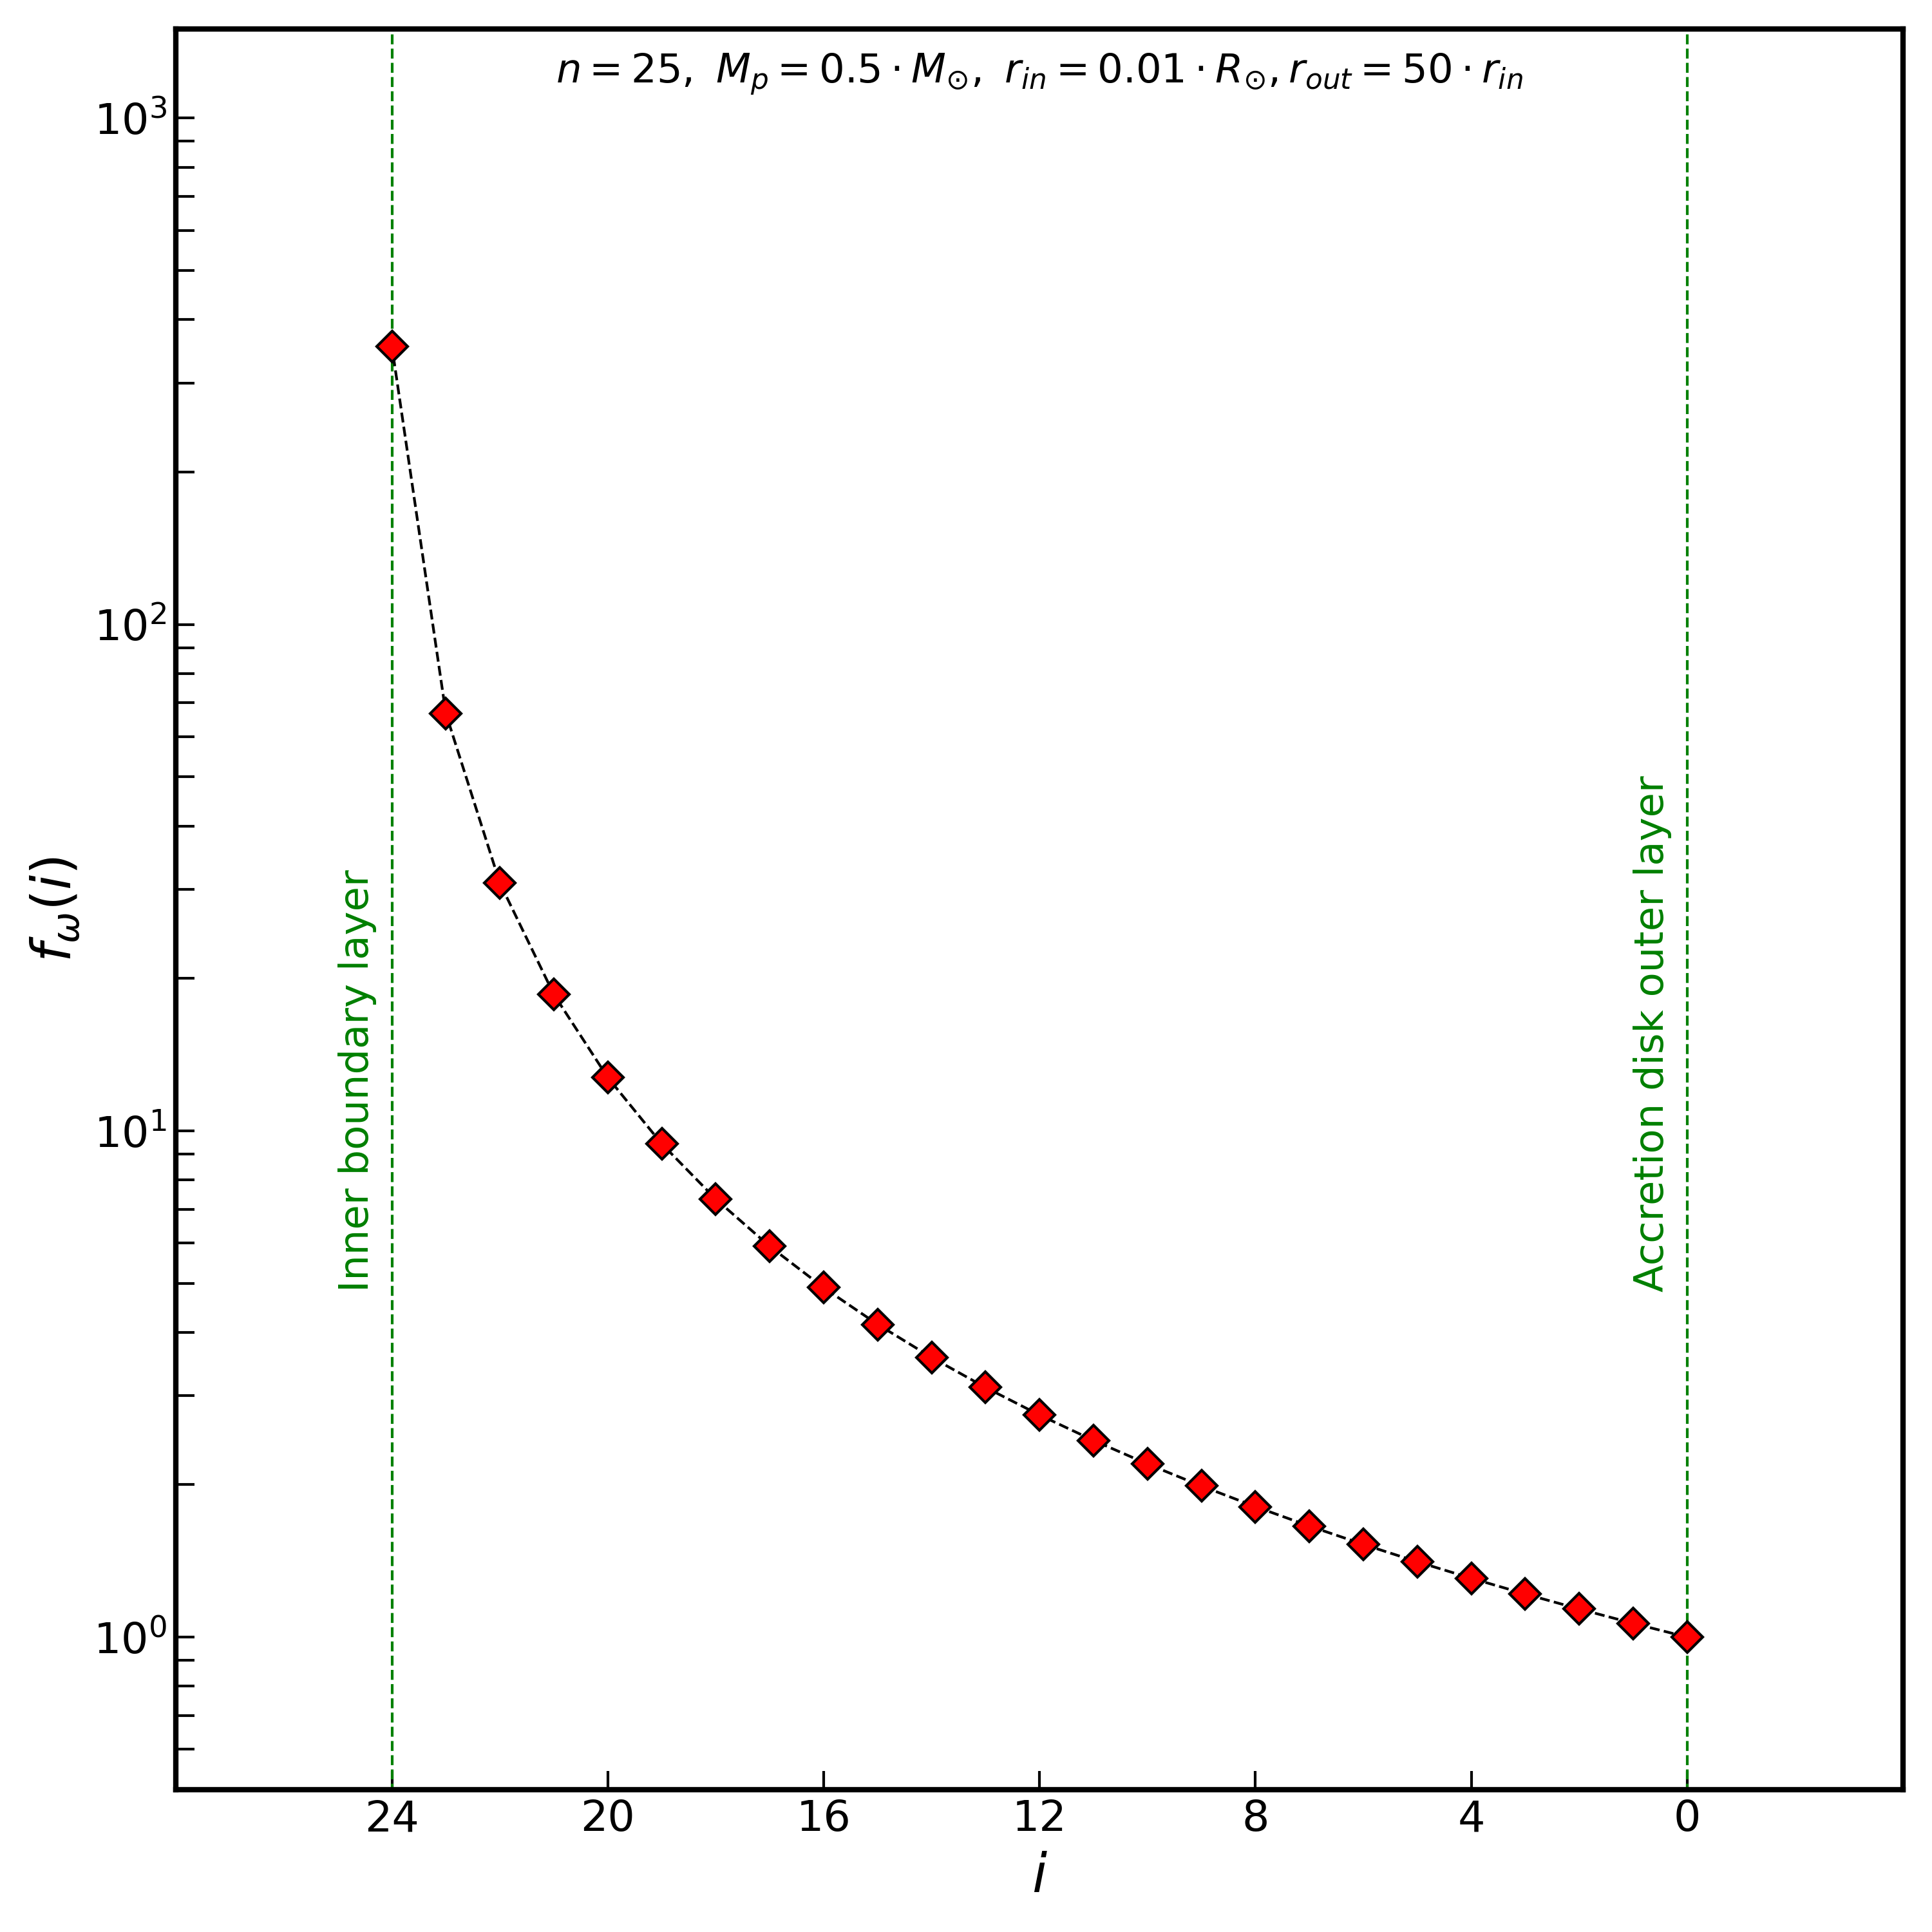
\includegraphics[width=0.9\columnwidth]{img/profile_omega.png}
\caption{Angular velocity profile relative to the layer $i = 0$ with modelled system parameters: $n=25$, $M_p = 0.5 \cdot M_{\odot}$, $r_{in} = 0.01 \cdot R_{\odot}$, $r_{out} = 50 \cdot r_{in}$}
\label{fig:profile_omega}
\end{figure}

\subsection{Gravity profile}

Similarly to angular velocity profile $f_{\omega}(i)$, the MDH model defines gravity profile $f_g(i)$, because the value of gravitational acceleration $g$ may differ by few orders of magnitude between central and outer regions of the accretion disc.  Value of $g_i$ for specific layer is:

\begin{equation} \label{eq:layer_g}
g_{i} = \frac{GM_{p}}{r_{i}^2},
\end{equation}

where $M_p$ represents mass of the central object, $G$ is the universal gravitational constant and $r_i$ is layer radius (i.e. distance to the center of gravity). Same as in the case of angular velocity profile $f_{\omega}(i)$ the gravity profile $f_g(i)$ is defined as relative value to the outermost layer $i = 0$ as:

\begin{equation} \label{eq:profile_g}
f_g(i) = \frac{g_i}{g_0}
\end{equation}

Substitution of equation \ref{eq:layer_g} into \ref{eq:profile_g} cancels out again the $GM_p$ term and gives the final form of gravity profile:

\begin{equation} \label{eq:profile_g_final}
f_g(i) = \left(\frac{r_{0}}{r_i}\right)^2=\left(\frac{r_{out}}{r_i}\right)^2.
\end{equation}

Figure \ref{fig:profile_g} shows example of such a profile and results of equation \ref{eq:profile_g_final} are later used in cell MSMM ODE system to describe the differing influence of central object on mass in specific cells. 

\begin{figure}[H]
\centering
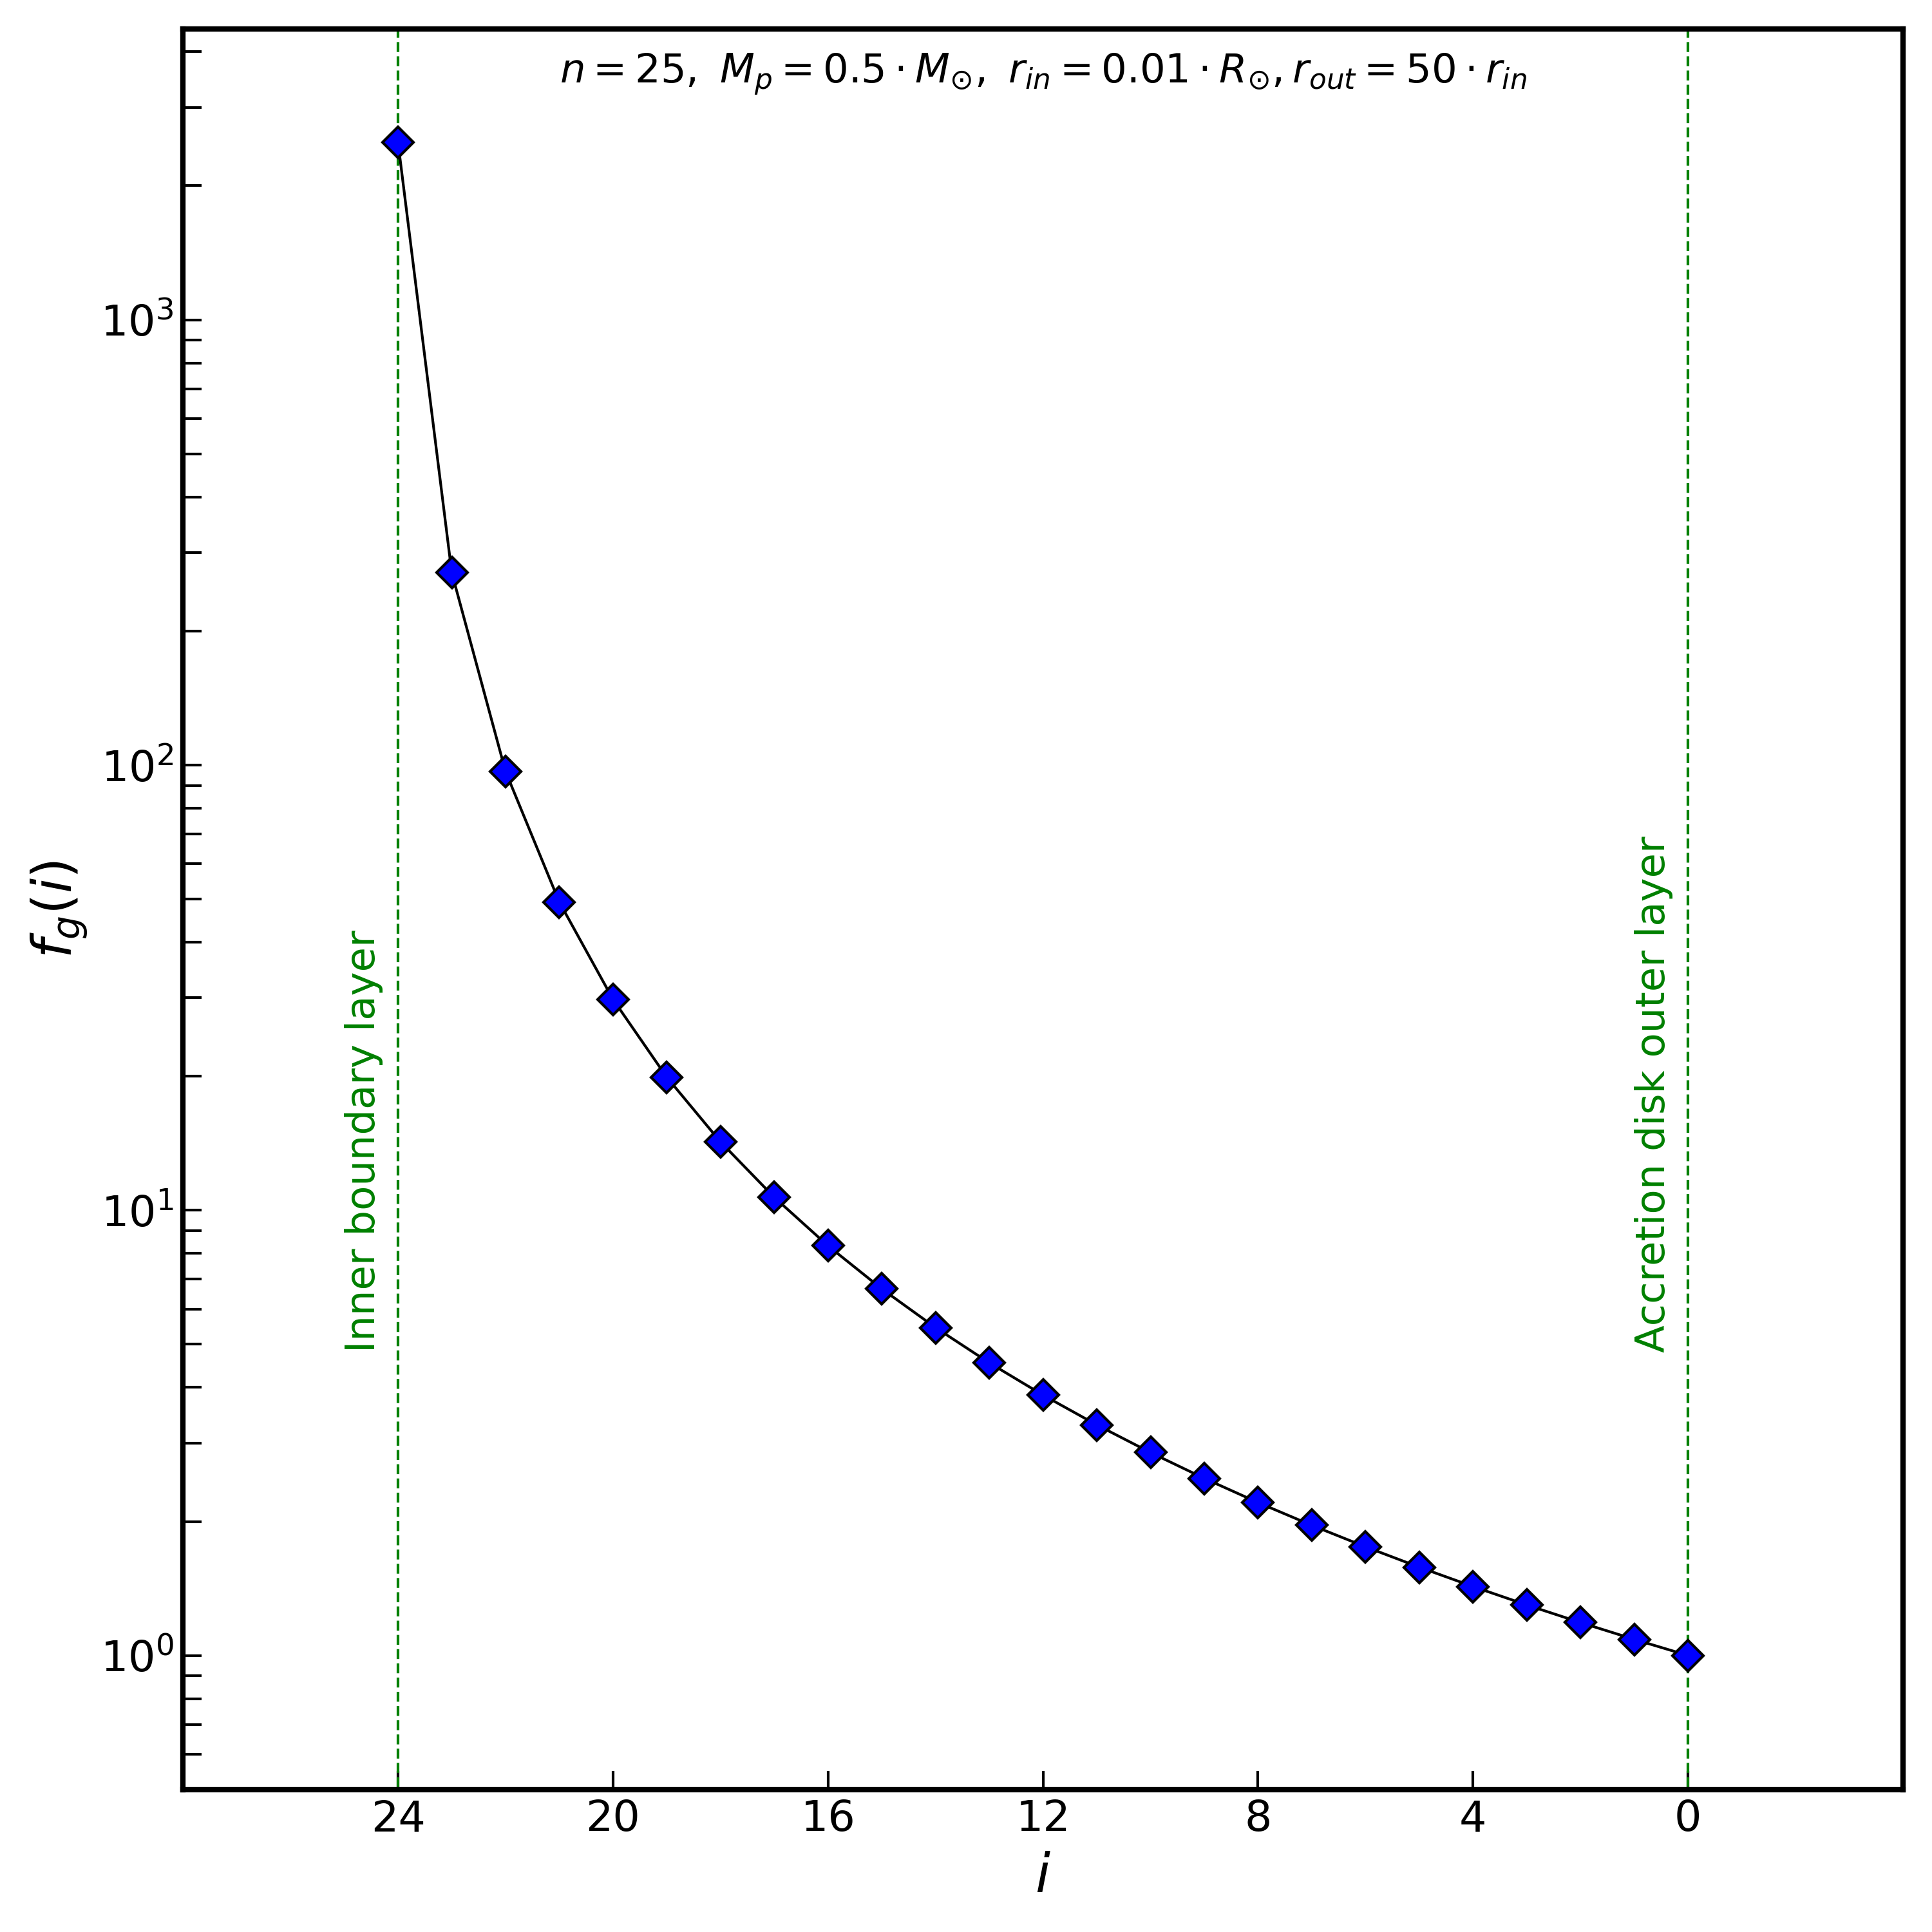
\includegraphics[width=0.9\columnwidth]{img/profile_g.png}
\caption{Gravity profile relative to the layer $i = 0$ with modelled system parameters: $n=25$, $M_p = 0.5 \cdot M_{\odot}$, $r_{in} = 0.01 \cdot R_{\odot}$, $r_{out} = 50 \cdot r_{in}$}
\label{fig:profile_g}
\end{figure}

\subsection{MSMM parameters}



MSMM ODE system ... 

\begin{equation}
    \D{}{t} \left(m \D{z}{t}\right) = -kz - \gamma\D{z}{t} + f_g(i) \cdot m,
\end{equation}
\begin{equation}
    \D{m}{t} = Q = const.,
\end{equation}

MSMM \emph{spring stiffness} ...

\begin{equation}
    \begin{aligned}
        & k~= 
        \begin{cases}
            -11{,}4m + 52{,}5 \hspace{10mm} (m < 4{,}61) \\
            \hspace{10mm} 0 \hspace{21mm} (m \ge 4{,}61 ),
        \end{cases}
    \end{aligned}
\end{equation}

Mass redistribution criteria ...

\begin{equation}
    m_r = 0.2m+0.3.
\end{equation}

\subsection{Temperature}

\section{Simulation}

Layer orbital period ...

\begin{equation}
    T_{i=0} = \sqrt{\frac{4 \pi^2 r_{out}^3}{G M_{p}}}.
\end{equation}

Time step size ...

\begin{equation}
    h = T_{i=0} / m,
\end{equation}




    
    % 9. MDH - THERMAL PROCESSES
    % \chapter{MDH - THERMAL PROCESSES}
\thispagestyle{empty}



    % 10. MDH - SYNTHETIC LIGHT CURVES
    % \chapter{MDH - SYNTHETIC LIGHT CURVES}
\thispagestyle{empty}


    % 11. MODELLING TECHNIQUES AND IMPLEMENTATION 
    \chapter{MDH -- MODEL IMPLEMENTATION}
\thispagestyle{empty}





    % 12. CV - MODEL
    \chapter{CV MODELS}
\thispagestyle{empty}

\mquote{640K ought to be enough for anybody}{Bill Gattes}


    % 13. ALPHA MODEL FITING
    \chapter{ALPHA MODEL FITING}
\thispagestyle{empty}


    % DISCUSSION
    \chapter{DISCUSSION}
\thispagestyle{empty}
\mquote{...}{...}

% TODO: napsat kapitolu
% TODO: citát! 

    Over the course of this publication we provided a detailed description of our \emph{Multilayer accretion disc} (MDH) model (see Chapter~\ref{chap:multilayer_dripping_handrail}), did an overview of its specific code implementation (see Chapter~\ref{chap:model_implementation}), nad demostrated its capabilities on chosen generic CV system using several model configurations (see Chapter~\ref{chap:cv_models}). We then used these results to obtain specific values of Shakura-Sunyaev $\alpha$ parameter for each configuration. 

    In this last Chapter, we would like to disscuss the successes, limitations or failures regarding the specific topics of our research journey with the MDH model. Also we want to provide some questions, ideas or inspirations for our future research or the related research of others.
    
\section{MDH implementation}

\section{Simulations results}

\section{Determining the Shakura-Sunyaev $\alpha$ parameter}

\section{Future research questions and inspiration}



    \pagestyle{plain}

    % Seznam použitých zkratek
    \newpage
\phantomsection
\addcontentsline{toc}{chapter}{LIST OF ABBREVIATIONS}
\noindent \Large \textbf{LIST OF ABBREVIATIONS}
\normalsize

\vspace{1cm}

\begin{center}
\def\arraystretch{1.5}%
\setlength\tabcolsep{1cm}
\begin{tabular}{ll}
    CV			& cataclysmic variable star \\
    WD			& white dwarf star \\
    NS          & neutron star \\
    BH          & black hole \\
    YSO         & young stelar object \\
    AGN         & active galactic nuclei \\
    XB          & X-ray binary \\
    HMXB        & high-mass X-ray binary \\
    LMXB        & low-mass X-ray binary \\
    FDM			& fluid dynamical model \\
    MSM			& mass-spring model \\
    MSMM		& mass-spring model modified \\
    CA			& cellular automaton \\
    ODE			& ordinary differential equation
\end{tabular}
\end{center}


    % Seznam použitých konstant
    \newpage

\phantomsection
\addcontentsline{toc}{chapter}{LIST OF CONSTANTS}
\noindent \Large \textbf{LIST OF CONSTANTS}
\normalsize

\vspace{10mm}
\begin{center}

\begingroup
\def\arraystretch{1.5}

\begin{tabularx}{\textwidth}{ccX}
\hline
\hline
\textbf{Symbol}	& \textbf{Value [units]} & \textbf{Meaning} \\
\hline
\hline
$G$	&
	\begin{tabular}{c}
        $6.67430 \cdot 10^{-11}\ [\si{\newton \cdot \meter^2 \cdot \kilogram^{-2}}]$ \\
         $6.67430 \cdot 10^{-8}\ [\si{\mathrm{dyne} \cdot \cm^2 \cdot \gram^{-1}}]$
	\end{tabular} 
	& Gravitational const. \\

$h$ &
	\begin{tabular}{c}
        $6.6260755 \cdot 10^{-34}\ [\si{\meter^2 \cdot \kilogram \cdot \second^{-1}}] $ \\
         $6.6260755 \cdot 10^{-27}\ [\si{\cm^2 \cdot \gram \cdot \second^{-1}}]$
	\end{tabular} 
	& Planck's const. \\
	
$k$ &
	\begin{tabular}{c}
        $1.380658 \cdot 10^{-23}\ [\si{\meter^2 \cdot \kilogram \cdot \second^{-2} \cdot \kelvin^{-1}}]$ \\
        $1.380658 \cdot 10^{-16}\ [\si{\mathrm{erg} \cdot \kelvin^{-1}}]$
	\end{tabular} 
	& Boltzmann's const. \\
	
$\sigma$ &
	\begin{tabular}{c}
        $5.670374 \cdot 10^{-8}\ [\si{\watt \cdot \meter^{-2} \cdot \kelvin^{-4}}] $ \\
        $5.670374 \cdot 10^{-5}\ [\si{\mathrm{erg} \cdot \cm^{-2} \cdot \gram^{-1} \cdot \second^{-2}}]$
	\end{tabular} 
	& Stefan-Boltzmann's const. \\

$c$ &
	\begin{tabular}{c}
        $2.99792458 \cdot 10^{8}\ [\si{\meter \cdot \second^{-1}}]$ \\
         $2.99792458 \cdot 10^{10}\ [\si{\cm \cdot \second^{-1}}]$
	\end{tabular} 
	& Speed of light \\
	
$M_{\odot}$	&
	\begin{tabular}{c}
        $1.98847\cdot 10^{30}\ [\si{\kilogram}]$ \\
         $1.98847\cdot 10^{33}\ [\si{\gram}]$
	\end{tabular} 
	& Solar mass \\

$R_{\odot}$	&
	\begin{tabular}{c}
        $6.957\cdot 10^{8}\ [\si{\m}]$ \\
        $6.957\cdot 10^{10}\ [\si{\cm}]$
	\end{tabular} 
	& Solar radius \\
	
\hline

\end{tabularx}

\endgroup

\end{center}


    % Sezman figures/grafu
    \newpage

\phantomsection
\addcontentsline{toc}{chapter}{LIST OF FIGURES}
\noindent \Large \textbf{LIST OF FIGURES}
\normalsize


    % Seznam literatury
    \newpage
\phantomsection
\addcontentsline{toc}{chapter}{REFERENCES}
\noindent \Large \textbf{REFERENCES}
\printbibliography[type=article,title={Articles},heading=subbibliography]
\printbibliography[type=book,title={Books},heading=subbibliography]
\printbibliography[type=thesis,title={Thesis},heading=subbibliography]
\printbibliography[type=misc,title={Miscellaneous},heading=subbibliography]

\end{document}
